
\chapter{Il sistema SADeB}

\medskip

Come già precedentemente indicato, il sistema {\tt SADeB} (Solid Authenticity Decentralized Blog), è formato dalle due applicazioni {\tt my-solid-blog} e {\tt blog-validator}.

\bigskip

\textbf{Vengono ora descritti nel dettaglio l'implementazione e le modalità di funzionamento dell'applicazione my-solid-blog.}

\bigskip

\section{Directory e file presenti in my-solid-blog}

\medskip


Come già accennato, {\tt my-solid-blog} è un'applicazione creata tramite il comando\\{\tt create-react-app} di {\tt npx}, il quale permette di sviluppare applicazioni in {\tt React} single-page. All'interno della directory principale sono presenti le seguenti cartelle:

\medskip

\begin{itemize}
	\item {\tt node-modules}: cartella contenente tutti i package scaricati tramite {\tt npm} per il progetto {\tt JavaScript} in questione. Alcuni di questi package sono stati scaricati nel momento in cui l'applicazione è stata creata tramite il comando {\tt create-react-app}, ad esempio quelli relativi a {\tt babel} o {\tt webpack}. Altri package, invece, sono stati successivamente aggiunti tramite il comando {\tt npm install}, come ad esempio: {\tt solid-client} e {\tt rdf-namespaces}.
	\item {\tt public}: La cartella {\tt public} contiene il file {\tt HTML} in modo da poterlo modificare, per esempio per impostare il titolo del progetto e alcuni metadati relativi all'applicazione. Le cartella {\tt public}, secondo la documentazione di {\tt React}, può essere utilizzata per uno dei seguenti casi:
	
	\medskip
	
	\textbf{1)} Se si hai bisogno di un file con un nome specifico nell'output di compilazione.\\
	\textbf{2)} Se sono presenti nel progetto migliaia di immagini e si ha la necessità di referenziare dinamicamente il loro percorso.\\
	\textbf{3)} Se si vuole includere in questa cartella un piccolo file {\tt JavaScript} lontano dagli altri file {\tt .js}.\\
	\textbf{4)} Se alcune librerie sono incompatibili con {\tt webpack} e vanno pertanto necessariamente incluse all'interno del file {\tt HTML}, tramite il tag {\tt <script>}.
	
	\medskip
	
	Nel caso specifico del progetto {\tt my-solid-blog}, la cartella {\tt public} è stata usata, oltre che per indicare il titolo e alcuni metadati relativi all'applicazione, per memorizzare l'icona di {\tt my-solid-blog}.
	
	\item {\tt src}: la cartella {\tt src} contiene tutti i principali file {\tt JavaScript} del progetto. Il file {\tt index.js}, creato direttamente dal comando\\{\tt create-react-app}, è l'entry point di {\tt JavaScript}.
	
	\medskip 
	
	Oltre ai file formato {\tt .js}, la cartella {\tt src} contiene anche il file {\tt CSS} per la formattazione del documento {\tt HTML} generato da {\tt React}.
	
	\medskip
	
	{\tt React} permette agli sviluppatori di riorganizzare la cartella {\tt src} in diverse sottocartelle per poter raggruppare alcuni file {\tt JavaScript} aventi caratteristiche in comune. Nel caso particolare di {\tt my-solid-blog}, sono presenti due sottocartelle chiamate {\tt components} e {\tt utils}.
\end{itemize}

\medskip

All'interno della directory principale del progetto, oltre a queste tre cartelle, sono presenti anche due file con le seguenti funzioni:

\begin{itemize}
	\item {\tt package-lock.json}: file che viene modificato a seguito di ogni operazione di {\tt npm} che vada a cambiare il contenuto della cartella {\tt node-modules} o il file {\tt package.json}. Descrive l'esatta struttura della cartella {\tt node-modules}.
	\item {\tt package.json}: file contenente importanti informazioni riguardo al progetto, come il nome del progetto stesso e una lista di dipendenze richieste da esso.
\end{itemize}

\bigskip

\section{Directory src}

\medskip

La cartella {\tt src}, come già detto, contiene tutti i file {\tt JavaScript} e {\tt CSS} per la creazione del documento {\tt HTML} da parte di {\tt React}: gestisce quindi l'impaginazione, la formattazione e stabilisce il comportamento dell'applicazione.

\medskip

All'interno di tale directory sono presenti i seguenti file {\tt JavaScript}:

\begin{itemize}
	\item {\tt index.js}: entry point di {\tt JavaScript}
	\item {\tt App.js}: file {\tt JavaScript} solitamente presente in progetti {\tt React}, all'interno di {\tt my-solid-blog} viene utilizzata per capire quale interfaccia grafica deve essere mostrata all'utente: {\tt App.js} si occupa di renderizzare un'interfaccia grafica diversa all'utente, una volta che quest'ultimo ha effettuato l'accesso all'interno dell'applicazione.
\end{itemize}

\medskip 

All'interno della cartella {\tt components}, sottocartella di {\tt src}, sono contenuti tutti i file {\tt JavaScript} che definiscono le varie interfacce utente utilizzate da {\tt my-solid-blog}. Nel dettaglio i file contenuti in {\tt components} sono:

\begin{itemize}
	\item {\tt ChoiceMenu.js}: Permette all'utente di scegliere se autenticarsi o inserire la {\tt webId} di un altro utente.
	\item {\tt EntryArea.js}: si occupa di renderizzare l'interfaccia grafica dell'applicazione quando l'utente non ha ancora effettuato l'accesso. In base alla scelta effettuata dall'utente, renderizza i componenti necessari per loggarsi con il proprio {\tt Solid Identity Provider}, oppure per poter inserire una {\tt webId} di un secondo utente.
	\item {\tt MainPage.js}: una volta effettuato l'accesso, si occupa di renderizzare le interfacce grafiche fornite da {\tt Header.js} e {\tt Articlelist.js}.
	\item {\tt Header.js}: renderizza nella parte superiore della pagina web alcune informazioni riguardanti l'utente proprietario del {\tt Pod}, come il nome, l'organizzazione a cui appartiene e il ruolo in tale organizzazione.
	\item {\tt Articleslist.js}: importando {\tt Article.js} renderizza l'intera lista di articoli presenti all'interno del {\tt Pod}. Nel caso in cui l'utente sia autenticato, renderizza anche l'interfaccia grafica fornita da {\tt WriteArticles.js}.
	\item {\tt Article.js}: Crea un'interfaccia grafica per mostrare il contenuto di un articolo, indicando titolo, testo e data. Inoltre, qualora l'utente sia autenticato, permette di modificare o cancellare un articolo.
	\item {\tt WriteArticles.js}: Permette di scrivere nuovi articoli all'interno del proprio {\tt Pod}.
\end{itemize}

\medskip

Oltre a {\tt components} è presente una seconda sottocartella chiamata {\tt utils}. Tale directory contiene i seguenti file:

\begin{itemize}
	\item {\tt GetOrCreateDataset}: tale file esporta una funzione necessaria per poter scaricare il dataset contenente gli articoli salvati all'interno del {\tt Pod}, chiamata\\{\tt getOrCreateDataset()}. Tale funzione controlla prima di tutto se esiste già un {\tt SolidDataset} all'interno del {\tt Pod}, in cui sono memorizzati gli articoli relativi all'utente; se questo esiste, allora viene correttamente scaricato, altrimenti tale {\tt SolidDataset} viene inizializzato dall'applicazione stessa.
	\item {\tt fontawesome.js}: file di secondaria importanza, permette di scaricare alcune icone dalle librerie {\tt fontawesome} per poterle utilizzare all'interno del progetto.
\end{itemize}

\bigskip

Oltre a queste cartelle e file, la directory {\tt src}, come già affermato, contiene anche i file necessari per la formattazione del documento {\tt HTML} generato. A tal proposito l'applicazione {\tt my-solid-blog} utilizza il framework {\tt CSS} {\tt Bulma}. 

\medskip

Il file {\tt index.scss}, il quale si occupa della formattazione del documento {\tt HTML} creato da {\tt my-solid-blog}, in accordo con la documentazione di {\tt Bulma}, importa solo i componenti del framework {\tt Bulma} utilizzati all'interno del progetto per la formattazione del documento {\tt HTML}. Inoltre modifica alcune variabili relative a tale framework e scarica i font utilizzati dall'applicazione.

\begin{figure}[ht]
	\centering
	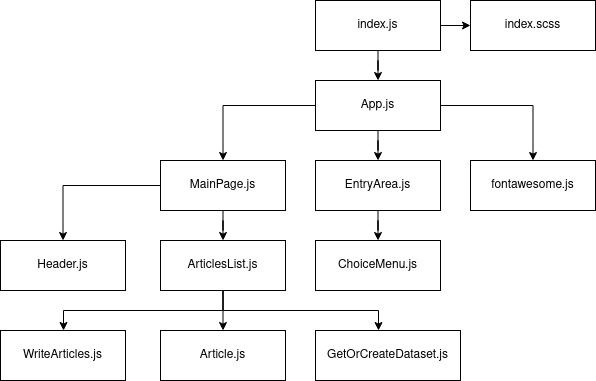
\includegraphics[width=0.87
	\textwidth,  keepaspectratio]{fig/Dependencies}
	\caption{L'albero delle dipendenze dei moduli di {\tt my-solid-blog} contenuti all'interno della directory {\tt src}.}
	\label{fig:bernersLee}
\end{figure}

\bigskip

\section{Gestione delle interfacce grafiche}

\medskip

Importante argomento all'interno di {\tt my-solid-blog} è quello riguardante la renderizzazione delle interfacce grafiche presenti all'interno del progetto. Infatti l'utente deve poter visualizzare differenti interfacce grafiche ad esempio in relazione al fatto che abbia già effettuato l'accesso o meno. 

\bigskip

{\tt React} effettua un rerender dei propri componenti ogni volta che lo stato di un componente cambia. A tale scopo è stato utilizzato l'{\tt hook} {\tt state} di {\tt React}, per poter andare a modificare lo stato dei vari componenti in base alle decisioni prese dall'utente all'interno dell'applicazione.

\bigskip

Innanzitutto va precisato che gli {\tt hooks} sono una feature di {\tt React} aggiunta recentemente; questa permette di utilizzare {\tt state} ed altre features caratteristiche di {\tt React} senza dover necessariamente scrivere una classe, come precedentemente richiesto. Al contrario utilizzando l'{\tt hook} {\tt state}, è stato possibile realizzare l'applicazione {\tt my-solid-blog} senza dover scrivere alcuna classe.

\bigskip

Viene qui di seguito riportato un esempio di codice per l'utilizzo dell'hook {\tt State}.

\medskip

\begin{lstlisting}

import React, { useState } from 'react';
 ... 
const [state, setState] = useState("")
 ... 
\end{lstlisting}

\medskip

La variabile {\tt state}, in questo esempio, rappresenta il valore attuale dello stato, mentre la funzione {\tt setState()} permette di modificare lo stato {\tt state}; il valore contenuto all'interno di {\tt useState()}, in questo esempio {\tt ""}, rappresenta il valore dello stato nel momento in cui tale componente viene caricato per la prima volta.

\bigskip

All'interno del progetto {\tt my-solid-blog}, tale hook è stato, per esempio, utilizzato in {\tt App.js}, per determinare quale interfaccia grafica mostrare all'utente in relazione al fatto che quest'ultimo abbia già completato la procedura di accesso o meno. Viene ora mostrato parte del codice contenuto nel modulo {\tt App.js}.

\medskip

\begin{lstlisting}
import React, { useState } from 'react';
...
function App () {
  const [entered, setEntered] = useState(false);
  const [webId, setWebId] = useState("");
  return (
    <div>
    { !session.info.isLoggedIn && !entered ? (
      <EntryArea
        entering={() => setEntered(true)}
        setWebId={(id) => setWebId(id)}
      />       
    ) : (        
      <MainPage
        webId={webId}
      />
    )}
    </div>
  );
}
\end{lstlisting}

\medskip

Il codice sopra mostrato è un perfetto esempio di come il problema di rerenderizzazione delle interfacce grafiche è stato affrontato all'interno dell'applicazione {\tt my-solid-blog}. In questo caso lo stato {\tt entered} è una variabile booleana pari a {\tt false} nel caso in cui l'utente debba ancora accedere all'applicazione e pari a {\tt true} altrimenti. Lo stato {\tt webId} serve invece per poter salvare la {\tt webId} del proprietario del blog da visualizzare, nel caso in cui non si voglia accedere al proprio blog autenticandosi. Se l'utente non ha ancora effettuato l'accesso all'applicazione, il modulo {\tt App.js} renderizza il componente $<EntryArea>$ che gestisce l'interfaccia grafica dell'applicazione prima di aver effettuato l'accesso, altrimenti viene renderizzato il componente $<MainPage>$ il quale contiene anche l'interfaccia grafica relativa ad ogni singolo articolo. La funzione $() => setEntered(true)$ viene passata al componente $<EntryArea>$ per permettergli di modificare lo stato {\tt entered} di {\tt App.js}. In questo modo {\tt EntryArea.js} può utilizzare tale funzione nel momento in cui l'utente ha effettuato l'accesso al blog appartenente ad una determinata {\tt webId} selezionata. Modificando lo stato {\tt entered}, {\tt EntryArea.js} forza {\tt App.js} a rerenderizzare la propria interfaccia grafica, in modo tale da visualizzare la lista di articoli presenti nel blog selezionato, renderizzando il componente $<MainPage>$.

\bigskip

\section{Container e risorse utilizzati per la gestione del blog}

\medskip

Dalle specifiche dell'applicazione {\tt my-solid-blog} risulta che i dati relativi agli articoli devono essere necessariamente pubblici, in quanto devono essere accessibili anche da parte utenti non autenticati. Infatti, nota la {\tt webId} di un utente, chiunque deve essere in grado di leggere il suo blog tramite l'applicazione {\tt my-solid-blog}.

\bigskip

Da tali considerazioni si evince che il {\tt container} ideale per salvare le informazioni inerenti al blog è il {\tt container} {\tt public}. Tale {\tt container} è normalmente presente di default in ogni {\tt Pod}. Le risorse {\tt ACL} di tale {\tt container} consentono di avere diritto in lettura sulle risorse all'interno di tale {\tt container}; questo significa che le risorse interne a tale {\tt container} possono essere scaricate anche senza essersi precedentemente autenticati con il server {\tt Solid}. Inoltre all'interno del {\tt container} {\tt setting}, anch'esso di norma presente di default all'interno del {\tt Pod}, è contenuto un {\tt SolidDataset} chiamato {\tt publicTypeIndex.ttl} avente lo scopo di tenere traccia di tutti i {\tt SolidDataset} accessibili pubblicamente all'interno del {\tt Pod}; anche la risorsa {\tt publicTypeIndex.ttl} è accessibile pubblicamente in lettura agli utenti non autenticati. L'applicazione {\tt my-solid-blog} salva il proprio {\tt SolidDataset}, chiamato {\tt articlelist.ttl}, all'interno di un {\tt container} chiamato\\ {\tt my-solid-blog}, creato dall'applicazione stessa, e situato a sua volta all'interno del {\tt container} {\tt public} per le considerazioni esposte in precedenza. Poiché {\tt articlelist.ttl} è una risorsa pubblicamente accessibile, {\tt my-solid-blog} riporta all'interno del {\tt SolidDataset} {\tt publicTypeIndex.ttl} alcune informazioni riguardanti {\tt articlelist.ttl}, tra le quali l'URL della risorsa per poterla scaricare tramite {\tt publicTypeIndex.ttl}. Infine l'applicazione legge anche alcuni dati contenuti direttamente all'interno del {\tt SolidDataset} relativo al profilo dell'utente. Il profilo di un utente è anch'esso una risorsa pubblicamente accessibile. Le informazioni lette dal profilo sono, ad esempio, il nome, l'organizzazione di cui fa parte l'utente e il ruolo che ha in tale organizzazione; queste informazioni vengono lette dall'applicazione per poterle mostrare all'utente insieme agli articoli contenuti all'interno del blog.

\bigskip

\section{Scaricamento del SolidDataset articlelist.ttl}

\medskip 

Nel momento in cui l'applicazione viene avviata, essa necessita di scaricare il {\tt SolidDataset} {\tt articlelist.ttl} dal {\tt Pod} dell'utente. I moduli che si occupano di eseguire queste operazioni sono {\tt ArticlesList.js} e {\tt GetOrCreateDataset.js}. Vengono qui di seguito elencate le operazioni eseguite da questi moduli per poter scaricare tale risorsa.

\begin{itemize}
	\item Per prima cosa è necessario conoscere la {\tt webId} dell'utente in questione. La {\tt webId} rappresenta l'URL dell'oggetto chiamato {\tt me} all'interno del profilo dell'utente sul quale vengono memorizzate le informazioni relative all'utente proprietario del {\tt Pod} e alla struttura del {\tt Pod} stesso. Se un utente si è autenticato con il {\tt Solid Identity Provider} allora l'applicazione può leggere la sua {\tt webId} utilizzando l'oggetto {\tt session} e in particolare la proprietà {\tt session.info.webId}. Se l'utente ha effettuato l'accesso senza autenticarsi, allora ha dovuto indicare la {\tt webId} dell'utente proprietario del blog che vuole leggere. Questo significa che, anche in questo caso, l'applicazione conosce la {\tt webId} da utilizzare.
	\item All'interno dell'oggetto {\tt me} è presente l'URL della radice del {\tt Pod}, necessario per poter conoscere l'ubicazione dei {\tt container} {\tt settings} e {\tt public}. Tale informazione è salvata utlizzando il vocabolario {\tt RDF} {\tt http://www.w3.org/ns/pim/space\#}, e in particolare, la proprietà {\tt storage} di tale vocabolario. Come descritto nel precedente capitolo, tale valore può essere letto utilizzando la funzione {\tt getUrl()}.
	\item Il vocabolario {\tt <http://www.w3.org/ns/solid/terms\#>}, ovvero il vocabolario di {\tt Solid}, viene utilizzato all'interno dell'oggetto {\tt me} per salvare l'URL del {\tt SolidDataset}\\ {\tt publicTypeIndex.ttl}; in particolare tale URL viene salvato utilizzando la proprietà {\tt publicTypeIndex} del vocabolario {\tt solid}.
	\item Viene scaricato il {\tt SolidDataset} {\tt publicTypeIndex.ttl}. Tale {\tt SolidDataset}, come in parte già accennato, contiene una lista di oggetti che si riferscono alle risorse accessibili pubblicamente all'interno del {\tt Pod}. L'applicazione usa {\tt publicTypeIndex.ttl} per controllare se esite un oggetto al suo interno che si riferisce ad {\tt articlelist.ttl}.
	\item Se esiste tale oggetto riferito ad {\tt articlelist.ttl}, questo significa che tale {\tt SolidDataset} esiste già all'interno del {\tt Pod}, cioè è stato creato in precedenza. In questo caso l'applicazione deve solamente leggere il valore sotto la proprietà {\tt instance} del vocabolario {\tt solid} per conoscere l'URL sotto il quale {\tt articlelist.ttl} è stato salvato. Una volta noto l'URL di {\tt articlelist.ttl}, l'applicazione può procedere scaricando tale {\tt SolidDataset}.
	\item Nel caso in cui tale oggetto non esista, questo significa che {\tt articlelist.ttl} non è stato inizializzato. L'applicazione deve quindi procedere creando tale risorsa.
	\item Viene quindi composto l'URL della risorsa {\tt articlelist.ttl} da creare, aggiungendo all'URL della radice del {\tt Pod}, precedentemente ottenuto utilizzando l'oggetto {\tt me}, la stringa "public/my-solid-blog/articlelist.ttl".
	\item Il {\tt SolidDataset} in questione viene creato sotto tale URL; tale operazione può essere compiuta solo se l'utente ha effettuato l'accesso all'applicazione completando l'operazione di logging. In caso contrario {\tt my-solid-blog} non possiede il diritto in scrittura necessario per effettuare tale operazione, ed è costretto ad arrestarsi, senza permettere all'utente di visualizzare alcun articolo.
	\item Come ultima operazione viene creato un oggetto all'interno di {\tt publicTypeIndex.ttl}, per poterci salvare l'URL scelto per {\tt articlelist.ttl}. In questo modo l'applicazione potrà utilizzare tale informazione la volta successiva in cui dovrà leggere tale blog per poter scaricare tale {\tt SolidDataset}.
\end{itemize}

\bigskip

\section{Struttura di articlelist.ttl}

\medskip

{\tt articlelist.ttl} contiene al suo interno vari oggetti, ognuno dei quali si riferisce ad un articolo differente pubblicato all'interno del {\tt Pod}. Nel momento in cui si accede all'interno di {\tt my-solid-blog}, l'applicazione permette all'utente di visualizzare la lista di articoli presenti all'interno di tale {\tt SolidDataset}. 

\medskip

I singoli articoli sono stati definiti utilizzando il vocabolario {\tt RDF} {\tt http://schema.org/}, in particolare sono state utilizzate le seguenti proprietà e classi di tale vocabolario.

\begin{itemize}
	\item Ogni oggetto-articolo è un'istanza della classe {\tt TextDigitalDocument}, classe definita, appunto, nel vocabolario {\tt schema}; tale classe ha lo scopo di rappresentare file composti prevalentemente da testo.
	\item La proprietà {\tt dataCreated}, viene utizzata per indicare la data di creazione dell'articolo.
	\item La proprietà {\tt headline} indica il titolo dell'articolo.
	\item La proprietà {\tt text} è utilizzato per poter salvare il contenuto di un articolo.
	\item Infine la proprietà {\tt identifier} viene utilizzata per poter identificare univocamente ogni articolo presente in {\tt articlelist.ttl}.
\end{itemize}

\medskip

Come indicato all'interno della lista delle specifiche, l'applicazione mostra all'utente il titolo, la data e il contenuto di ogni articolo. L'identifier viene invece utilizzato come chiave di {\tt React}, per poter permettere a {\tt React} di renderizzare correttamente la lista di articoli presenti. Infine, su richiesta dell'utente, {\tt my-solid-blog} visualizza all'utente l'URL in cui la risorsa relativa al singolo articolo è stata memorizzata. Tale funzione, come verrà spiegato in seguito, è necessaria per permettere all'utente di interagire correttamente con il server {\tt blog-validator}.
\bigskip

\section{Gestione degli articoli}

\medskip

Come già in parte accennato, i moduli che si occuppano di gestire e renderizzare la lista di articoli presenti all'interno del blog sono: {\tt ArticlesList.js} e {\tt Article.js}.

\bigskip

Nel dettaglio {\tt Articleslist.js} si occupa di scaricare il {\tt SolidDataset}\\{\tt Articlelist.ttl}, di renderizzare e gestire la lista di articoli presenti importando {\tt Article.js}, di aggiungere nuovi articoli alla lista per gli utenti autenticati, di definire le funzioni per poter modificare o eliminare un articolo e di passare alcune informazioni come parametri necessari alla gestione dei singoli articoli ad {\tt Article.js}.

\bigskip

Il modulo {\tt Article.js} invece ha i seguenti compiti: renderizzare i singoli articoli contenuti all'interno del blog, utilizzare le funzioni definite in {\tt ArticlesList.js} per permettere agli utenti autenticati di modificare o cancellare un articolo, consentire a {\tt my-solid-blog} e {\tt blog-validator} di comunicare tra di loro per verificare l'autenticità dei singoli articoli mostrati da {\tt my-solid-blog}.

\bigskip

Una volta caricato il {\tt SolidDataset} {\tt Articlelist.ttl}, il modulo {\tt ArticlesList.js} utilizza la funzione {\tt getThingAll()} della libreria {\tt solid-client} per poter ottenere un array contenente tutti gli articoli del blog. Tale array viene quindi ordinato in base alla data di creazione degli articoli stessi, utilizzando la funzione {\tt byDate()}, anch'essa definita all'interno di {\tt ArticlesList.js}. Una volta che tale operazione è terminata, viene eseguito il metodo {\tt map()} sull'array precedentemente ottenuto, in modo tale da renderizzare il contenuto dei singoli articoli utilizzando il modulo {\tt Article.js}; tale funzione {\tt map()} ritorna il singolo componente $<Article>$ per ogni elemento presente all'interno dell'array. Al componente $<Article>$ vengono passati i seguenti argomenti:

\begin{itemize}
	\item {\tt thing}: oggetto rappresentante il singolo articolo all'interno del blog; tramite esso è possibile leggere e modificare le informazioni relative al singolo articolo.
	\item {\tt remove}: funzione che permette all'utente autenticato di eliminare un articolo all'interno del blog. Questa funzione asincrona riceve in ingresso l'oggetto, ovvero l'articolo, da eliminare da {\tt articlelist.ttl}; una volta eliminato la funzione salva all'interno del {\tt Pod} il {\tt SolidDataset} aggiornato.
	\item {\tt change}: funzione asincrona avente lo scopo di modificare il contenuto di un articolo: in particolare permette all'utente autenticato di modificare titolo e contenuto dell'articolo. Riceve in ingresso l'oggetto da modificare, il nuovo titolo e il nuovo contenuto. Una volta che l'articolo viene aggiornato la funzione salva all'interno del {\tt Pod} il {\tt SolidDataset} aggiornato.
	\item {\tt webId}: variabile contenente la {\tt webId} del proprietario del blog. Tale variabile viene utilizzata solamente se l'utente ha effettuato l'accesso senza autenticarsi; in caso contrario la {\tt webId} può essere letta direttamente da {\tt session.info.webId}.
\end{itemize}

\bigskip

{\tt Article.js} mette quindi a disposizione due componenti $<button>$ per permettere all'utente di modificare ed eliminare l'articolo renderizzato; tali componenti vengono visualizzati dall'utente solo se la variabile {\tt session.info.isLoggedIn} è pari a {\tt true}, cioè solamente se l'utente si è correttamente autenticato con il proprio {\tt Solid Identity Provider}.

\bigskip


\section{Comunicazione con l'applicazione blog-validator}

\medskip

Per effettuare un controllo sull'autenticità dei contenuti mostrati all'interno del blog dell'utente, l'applicazione {\tt my-solid-blog} comunica attraverso il protocolo {\tt HTTP} con il server {\tt blog-validator}.

\bigskip

A tale proposito viene utilizzato il metodo {\tt POST} per effettuare una richiesta a\\{\tt blog-validator}, dopodichè {\tt my-solid-blog} aspetta la risposta del server per poter mostrare all'utente l'esito di tale controllo.

\bigskip


Per inviare tale richiesta {\tt POST} al server, come già esposto all'interno del capitolo 2, l'applicazione {\tt my-solid-blog} fa uso della libreria {\tt axios}; in particolare utilizza il metodo {\tt axios.post()}; tale metodo ritorna all'applicazione una promessa. L'applicazione\\{\tt my-solid-blog} rimane in attesa che tale promessa si risolva o venga rifiutata. Nel caso in cui si risolva, allora questo significa che la comunicazione con il server è andata a buon fine. In questo caso l'applicazione può quindi mostrare all'utente l'esito del controllo effettuto da {\tt blog-validator}; in caso contrario, qualora la promessa venga rifiutata, si è verificato un errore durante tale comunicazione.

\bigskip

Per poter comunicare l'applicazione {\tt my-solid-blog} utilizza la porta {\tt 3000}, mentre {\tt blog-validator} utilizza la porta {\tt 8081}. Gli argomenti passati alla funzione {\tt axios.post()} sono i seguenti: l'URL su cui il server è in ascolto, che è pari a {\tt http://localhost:8081/auth} e tutte le informazioni necessarie al server per effettuare tale controllo attraverso un file formato {\tt JSON}. In particolare le proprietà presenti all'interno di tale file JSON sono le seguenti:

\begin{itemize}
	\item {\tt webId}: viene passata a {\tt blog-validator} la {\tt webId} del proprietario del {\tt Pod}. La {\tt webId} del proprietario è necessaria a comprendere se il server ha cercato le informazioni all'interno del {\tt Pod} corretto.
	\item {\tt urlDataset}: URL relativo al {\tt SolidDataset} da scaricare; {\tt my-solid-blog} invia, infatti, a {\tt blog-validator} l'URL relativo a {\tt articlelist.ttl}, per poterlo scaricare e poter leggere i dati al suo interno.
	\item {\tt urlThing}: URL in cui la risorsa relativa all'articolo è stata memorizzata, permette al server di trovare l'articolo in questione all'interno del {\tt SolidDataset}, nel caso in cui questo esista effettivamente all'interno di {\tt articlelist.ttl}.
	\item {\tt title}: titolo dell'articolo, necessario per controllare che questo non sia stato alterato da {\tt my-solid-blog}.
	\item {\tt content}: contenuto dell'articolo, inviato per le stesse motivazioni della proprietà {\tt title}.
	\item {\tt date}: data di creazione dell'articolo; è necessario inviare tale informazione per controllare che anche questo dato non sia stato manomesso in nessun modo dall'applicazione.
\end{itemize}

\bigskip

L'applicazione invia tale richiesta {\tt POST} a {\tt blog-validator} ogni volta che si preme il pulsante chiamato {\tt Check}, situato al di sotto di ogni articolo renderizzato da {\tt my-solid-blog}. L'esito del controllo viene anch'esso stampato al di sotto dell'articolo controllato.


\bigskip

\section{Utilizzo dell'hook Effect}

\bigskip

Oltre all'{\tt hook} {\tt State}, l'aplicazione {\tt my-solid-blog} utilizza un altro {\tt hook} di {\tt React}, chiamato {\tt Effect}, anch'esso aggiunto recentemente. Tale {\tt hook} è utilizzato per implementare side effects all'interno dei componenti delle funzioni. Esempi di side effects  all'interno dei componenti {\tt React} sono: il download di dati, l'impostazione di una iscrizione o il cambiamento manuale del {\tt DOM}.

\bigskip

Talvolta, quando si utilizza {\tt React} è necessario eseguire del codice aggiuntivo, dopo che {\tt React} ha aggiornato il {\tt DOM}. {\tt useEffect} serve ad informare i vari componenti {\tt React}, su cosa questi sono tenuti a fare una volta terminata l'operazione di renderizzazione delle interfacce grafiche. {\tt React} memorizza la funzione passata a questo {\tt hook} e la esegue in un secondo momento, ovvero dopo che il {\tt DOM} è stato aggiornato. Il codice all'interno {\tt useEffect} viene di default eseguito ogni volta che {\tt React} termina l'operazione di render. Questo hook è utilizzato all'interno di {\tt my-solid-blog} per scaricare il {\tt SolidDataset} {\tt articlelist.ttl}; infatti scaricare dati dalla rete è un tipico side effect da eseguire tramite {\tt Effect}. Per chi ha familiarità con le classi {\tt React}, l'{\tt hook} {\tt useEffect} sostituisce i metodi {\tt componentDidMount}, {\tt componentDidUpdate } e {\tt componentWillUnmount} delle classi {\tt React}.

\bigskip

Nel caso di {\tt my-solid-blog}, viene passata all'{\tt hook} {\tt useEffect} non solo la funzione da eseguire, ma anche l'array {\tt [session]}. Questo permette di ottimizzare l'applicazione, in quanto, passando questo argomento, la funzione all'interno di {\tt useEffect} non viene più eseguita al termine di ogni renderizzazione da parte di {\tt React}, ma soltanto quando uno o più elementi dell'array {\tt [session]}, fra un render e l'altro, sono cambiati.

\bigskip

\section{Link a blog-validator}

\medskip

All'interno dell'applicazione, come già precedentemente detto, è possibile inviare, tramite procollo {\tt HTTP}, una richiesta {\tt POST} al server {\tt blog-validator}, con il fine di evitare la diffusione di informazioni false all'interno dell'applicazione {\tt my-solid-blog}. Per effettuare tale controllo {\tt my-solid-blog} invia a {\tt blog-validator} alcune informazioni riguardanti i dati relativi all'articolo in questione. Una volta terminata la comunicazione con il server, l'applicazione {\tt my-solid-blog}, infine mostra all'utente l'esito del controllo effettuato da {\tt blog-validator}. Tuttavia l'utente, non avendo modo di vedere in prima persona i dati scambiati tra le due applicazioni, non può avere certezze riguardo i seguenti aspetti:

\begin{itemize}
	\item L'utente non può verificare se l'applicazione {\tt my-solid-blog} abbia effettivamente inviato correttamente i dati relativi all'articolo in questione. {\tt my-solid-blog} potrebbe inviare intenzionalmente dati relativi ad un altro articolo, per poter andare a modificare l'esito del controllo effettuato da {\tt blog-validator}.
	\item L'applicazione {\tt my-solid-blog} potrebbe far credere all'utente che {\tt blog-validator} non abbia rilevato anomalie durante il controllo, visualizzando a questo un esito differente da quello effettivamente rilevato dal server.
\end{itemize}

\medskip

Per evitare tale problema all'interno dell'applicazione {\tt my-solid-blog} è possibile trovare un link per potersi connettere direttamente con {\tt blog-validator} tramite browser. Visitando tale URL, l'utente può vedere quali sono stati realmente i dati inviati da {\tt my-solid-blog} a {\tt blog-validator} insieme al reale esito di tale controllo. In questo modo l'utente può verificare in prima persona se il controllo sull'autenticità degli articoli mostrati da {\tt my-solid-blog} può ritenersi valido o meno.

\clearpage

\textbf{Vengono ora descritte le modalità di funzionamento e l'implementazione dell'applicazione blog-validator.}

\bigskip

{\tt blog-validator} è un server implementato tramite {\tt Node.js}, utilizzato per controllare l'autenticità dei dati mostrati dall'applicazione {\tt my-solid-blog}; {\tt blog-validator} utilizza la porta 8081.

\bigskip


\section{Directory e file presenti in blog-validator}

\medskip

Sono qui di seguito elencati tutti i file e le directory presenti all'interno del progetto {\tt blog-validator}.

\medskip

La cartella {\tt node-modules} e i file {\tt package-lock.json} e {\tt package.json}, presenti all'interno dell'applicazione {\tt blog-validator}, sono già stati trattati in quanto presenti anche all'interno del progetto {\tt my-solid-blog}; per questo motivo non verranno ripetute le loro funzioni all'interno di questa sezione.

\begin{itemize}
	\item {\tt index.js}: file entry point {\tt JavaScript} del progetto {\tt blog-validator}. Definisce alcuni URL per effettuare richieste {\tt GET} e {\tt POST} da parte di terze applicazioni.
	\item {\tt solid.db}: Database utilizzato da {\tt blog-validator} per salvare alcuni dati 
	necessari per il funzionamento dell'applicazione.
	\item {\tt utils}: Directory contenente i moduli {\tt solidRequest.js} e {\tt requestsData.js}.
	\item {\tt solidRequest.js}: File utilizzato per leggere alcuni dati all'interno del {\tt Pod} dell'utente. La lettura di tale dati è necessaria per poter effettuare controlli riguardanti l'autenticità dei dati visualizzati da {\tt my-solid-blog}.
	\item {\tt requestsData.js}: Modulo per la gestione del database {\tt solid.db}, si occupa della creazione di tabelle, dell'inserimento di tuple, e della lettura di alcuni dati all'interno di tale database.
\end{itemize}

\medskip

\bigskip

\section{Tecnologie utilizzate per il funzionamento di blog-validator}

\medskip

Vengono ora brevemente descritti alcuni moduli fondamentali per il funzionamento del server {\tt blog-validator}.

\clearpage

\textbf{Express}

\bigskip

{\tt Express} è un framework per applicazioni web Node.js che fornisce una serie di funzioni avanzate per le applicazioni web e per dispositivi mobili; è ormai definito come il server framework standard de facto per {\tt Node.js}. Tale framework permette la creazione di {\tt API} in maniera semplice e veloce.

\bigskip

\textbf{cookie-session}

\bigskip

I {\tt Session cookies} sono i cookie temporanei che vengono generati principalmente sul lato server, il cui uso principale è quello di tenere traccia di tutte le informazioni della richiesta che è stata fatta dal cliente in una particolare sessione. La sessione viene memorizzata solo temporaneamente, quando l'utente chiude la sessione del browser costui la distrugge in automatico. 

\medskip

Il modulo {\tt express-session} chiamato {\tt cookie-session} è usato per la gestione delle sessioni in {\tt Node.js}.

\bigskip

\textbf{body-parser}

\bigskip

{\tt body-parser} è una libreria {\tt npm} usata per processare i dati inviati al server attraverso un metodo di richiesta {\tt HTTP}.

\bigskip

\textbf{sqlite3}

\bigskip

Libreria {\tt npm} utilizzata per la creazione e la gestione del database utilizzato da {\tt blog-validator}.

\bigskip

\section{API methods di blog-validator}

\medskip

Vengono ora elencati gli API methods messi a disposizione da {\tt blog-validator}.

\begin{itemize}
	\item {\tt POST}, {\tt http://localhost:8081/auth}: Questo metodo è utilizzato dall'applicazione {\tt my-solid-blog} per inviare al server i dati necessari a controllare i dati richiesti dall'utente. I dati ricevuti da {\tt my-solid-blog} vengono poi passati al modulo {\tt solidRequest.js}, il quale si occupa di confrontare le informazioni ricevute con quelle presenti all'interno del {\tt Pod}. I dati inviati da {\tt my-solid-blog} vengono salvati nel database {\tt solid.db}.
	\item {\tt GET}, {\tt http://localhost:8081/check}: Tale metodo è utilizzato per permettere all'utente di interagire con l'applicazione. Consente all'utente di controllare un articolo, una volta noti gli URL del suo {\tt SolidDataset} e dell'articolo stesso, o di controllare il corretto svolgimento di un controllo sull'autenticità dei dati effettuato da {\tt blog-validator} attraverso l'API method {\tt POST}, {\tt http://localhost:8081/auth}, con il fine di verificare che {\tt my-solid-blog} non abbia inviato al server dati scorretti.
	\item {\tt POST}, {\tt http:localhost:8081/control}: Metodo utilizzato per inviare all'utente i dati relativi al controllo sul quale è stata richiesta una verifica. Attraverso il modulo {\tt requestsData.js}, utilizza il database {\tt solid.db} per caricare tali dati richiesti.
	\item {\tt POST}, {\tt http:localhost:8081/read}:  Metodo utilizzato per inviare all'utente i dati relativi ad un articolo, ovvero titolo, contenuto e data di pubblicazione, salvato all'interno del {\tt Pod}. Tale metodo può essere utilizzato per verificare che tali dati coincidano con quelli visualizzati da {\tt my-solid-blog}.
\end{itemize}

\bigskip

\section{Controllo sull'autenticità dei dati}

\medskip

Viene ora descritto nel dettaglio il procedimento, effettuato da {\tt blog-validator}, per controllare l'autenticità dei dati riguardanti un articolo mostrato dall'applicazione {\tt my-solid-blog}. L'articolo sul quale effettuare il controllo viene scelto direttamente dall'utente che sta utilizzando {\tt my-solid-blog}.

\begin{itemize}
	\item Come già indicato precedentemente, quando un utente che sta utilizzando l'applicazione {\tt my-solid-blog} preme il pulsante "Check", {\tt my-solid-blog} invia una richiesta {\tt POST} utilizzando il metodo {\tt http://localhost:8081/auth}. {\tt blog-validator} riceve quindi tutti i dati necessari per verificare l'autenticità dell'articolo, selezionato dall'utente, mostrato da {\tt my-solid-blog}.
	\item I dati ricevuti vengono passati alla funzione {\tt readSolidData()} esportata dal modulo {\tt solidRequest.js}.
	\item Poiché l'applicazione {\tt my-solid-blog} ha passato al server la proprietà {\tt urlDataset}, il quale indica l'URL ove è situato il {\tt SolidDataset} contente l'articolo da controllare, {\tt readSolidData()} può scaricare tale {\tt SolidDataset} utilizzando le funzioni messe a disposizione dalla libreria di {\tt Inrupt} {\tt solid-client}. 
	\item Una volta scaricato il {\tt SolidDataset} in questione, attraverso la proprietà {\tt urlThing}, anch'essa ricevuta da {\tt my-solid-blog}, la quale rappresenta l'URL corrispondente all'articolo in questione, {\tt readSolidData()} può andare a cercare l'oggetto all'interno del {\tt SolidDataset} scaricato che si riferisce a tale articolo.
	\item Se l'articolo in questione non esiste {\tt blog-validator} restituisce a {\tt my-solid-blog}:
	
	\smallskip
	
	{\tt "Article not found: " + req.body.webId + " is not the author"}
	\item Se, invece, l'articolo esiste all'interno del {\tt Pod}, {\tt readSolidData()} legge il titolo e il contenuto di tale articolo e li confronta con quelli che ha ricevuto da {\tt my-solid-blog}.
	\item Se il titolo e/o il contenuto dell'articolo non corrispondono a quelli inviati da {\tt my-solid-blog}, {\tt blog-validator} restituisce a {\tt my-solid-blog} la seguente risposta:
	
	\smallskip
	
	{\tt "Article of " + req.body.webId + " found, but the title or the content are different"}
	\item Se il titolo e il contenuto dell'articolo corrispondono a quelli ricevuti da {\tt my-solid-blog}, {\tt readSolidData()} confronta la data di pubblicazione dell'articolo con quella ricevuta da {\tt my-solid-blog}.
	\item Se queste non corrispondono, {\tt blog-validator} invia a {\tt my-solid-bog} la risposta:
	
	\smallskip
	
	{\tt "Article of " + req.body.webId + " found, but the date is different, the real date is: " + date}
	\item Se c'è corrispondenza anche sulla data di pubblicazione dell'articolo allora {\tt blog-validator} invia a {\tt my-solid-blog} come risposta:
	
	\smallskip
	
	{\tt "Article of " + req.body.webId + " found, all in order"}
	
	\smallskip
	
	Arrivati a questo punto {\tt blog-validator} ha quindi terminato di controllare l'autenticità dell'articolo in questione.	
\end{itemize}

\medskip

Il corretto funzionamento della procedura sopra descritta è stata testata tramite il programma {\tt Postman}.

\bigskip

\section{Gestione del database solid.bd}

\medskip

{\tt blog-validator}, a seguito delle operazioni sopra descritte, utilizza la libreria {\tt sqlite3}, per salvare all'interno del database {\tt solid.db} i dati relativi alle richieste che sono state effettuate da {\tt my-solid-blog}. Tale database è molto semplice e presenta un'unica tabella chiamata {\tt userAuth}; all'interno di questa vengono salvate le informazione necessarie per permettere all'utente di verificare in prima persona che la comunicazione tra {\tt blog-validator} e {\tt my-solid-blog} sia avvenuta correttamente, senza che i dati relativi a tale comunicazione siano stati volontariamente manipolati da quest'ultima applicazione.

\bigskip

Ogni tupla della tabella {\tt userAuth} rappresenta un singolo controllo richiesto dall'applicazione {\tt my-solid-blog} attraverso il metodo {\tt POST} : {\tt http://localhost:8081/auth}. All'interno della tabella {\tt userAuth} sono presenti i seguenti attributi:

\begin{itemize}
	\item {\tt webId}: la {\tt webId} del proprietario del blog.
	\item {\tt urlDataset}: URL del {\tt SolidDataset} dove è memorizzato il blog. Tale {\tt SolidDataset} corrisponde con il Dataset {\tt articlelist.ttl} precedentemente trattato.
	\item {\tt urlThing}: URL corrispondente all'articolo sul quale è stato richiesto il controllo.
	\item {\tt title}: titolo dell'articolo.
	\item {\tt content}: contenuto dell'articolo.
	\item {\tt date}: data di pubblicazione dell'articolo.
	\item {\tt checkDate}: data nella quale è stato richiesto il controllo dall'utente.
	\item {\tt result}: esito del controllo.
\end{itemize}

Tutti i seguenti attributi elencati sono di tipo {\tt TEXT}.

\bigskip 

\section{Il metodo GET, http://localhost:8081/check}

\medskip

Utilizzando l'API method {\tt GET, http://localhost:8081/check} l'utente ha modo di visualizzare i dati contenuti in tale database. Tale link, come già precedentemente indicato, è presente anche all'interno dell'applicazione {\tt my-solid-blog}. Visitandolo un utente può inserire l'URL relativo ad un articolo per poter visualizzare i dati, salvati all'interno del database, relativi al controllo più recente che è stato richiesto su tale articolo. In alternativa, come già indicato, l'utente può digitare l'URL di un articolo e del {\tt SolidDatatset} in cui è salvato, per controllare manualmente il contenuto di tale articolo.

\bigskip

Il motivo per cui {\tt my-solid-blog} mette a disposizione dell'utente il link\\{\tt http://localhost:8081/check} è quello di provare a quest'ultimo che l'applicazione sta rispettando i criteri relativi alla tecnologia {\tt Solid}: l'applicazione, infatti, non salva localmente nessun dato relativo all'utente, ma utilizza unicamente i dati contenuti all'interno del {\tt Pod} dell'utente proprietario del blog.

\bigskip

\section{Possibili futuri miglioramenti del sistema SADeB}

\medskip

In questa sezione sono elencate alcune ulteriori funzionalità del sistema {\tt SADeB} che, per alcune motivazioni, non sono state implementate.

\begin{itemize}
	\item Quando si effettua un controllo su un articolo, {\tt my-solid-blog} potrebbe inviare a {\tt blog-validator} soltanto l'hash relativo al titolo e al contenuto di un articolo. Utilizzando, per esempio, l'algoritmo {\tt SHA-256}, il quale permette di generare {\tt digest} di lunghezza 256 bit per comunicare con il server {\tt blog-validator}, la comunicazione attraverso il protocollo {\tt HTTP} risulterebbe essere più veloce. In questo caso al server basterebbe soltanto confrontare l'hash inviatogli da {\tt my-solid-blog} con quello del titolo o del contenuto dell'articolo, per stabilire l'autenticità o meno dei contenuti postati all'interno del blog.
	\item Poiché {\tt Solid} permette ai propri utenti di memorizzare anche file all'interno del proprio {\tt Pod}, l'applicazione {\tt my-solid-blog} potrebbe in futuro permettere agli utenti di caricare un'immagine per il proprio blog, salvandola nel {\tt Pod}, e di consentire di visualizzarla ogni volta che un qualsiasi altro utente visiti il profilo. Attualmente {\tt Inrupt} mette a disposizione alcune funzioni all'interno della libreria {\tt solid-client} per poter leggere e scrivere file contenuti nel proprio {\tt Pod}.
	\item L'applicazione {\tt blog-validator} potrebbe memorizzare i dati relativi ai controlli richiesti dal client tramite la tecnologia {\tt Solid}, anziché utilizzare un {\tt database} locale. In questo caso sarebbe necessario trovare uno o più vocabolari {\tt RDF} per poter rappresentare tale tipologia di dati. Nel caso in cui non esistessero vocabolari adatti a tale scopo, sarebbe necessario scriverne uno e pubblicarlo all'interno del {\tt container} {\tt public} presente all'interno del {\tt Pod}. In questo modo il vocabolario risulterebbe accessibile ed utilizzabile anche da altri utenti che hanno la necessità di rappresentare la stessa tipologia di dati descritta all'interno di tale ipotetico vocabolario.
	\item L'applicazione {\tt my-solid-blog} potrebbe permettere di creare blog appartenenti a gruppi di utenti, anziché ad uno singolo; in questo caso il blog sarebbe formato dai vari articoli appartenenti agli utenti. Attraverso il vocabolario {\tt ACL}, che {\tt Solid} utilizza per determinare i livelli di permesso concessi ad un utente o ad un'applicazione all'interno di un {\tt Pod}, ogni utente potrebbe decidere quali altre persone oltre a lui possano modificare gli articoli presenti nel proprio {\tt SolidDataset} riferito al {\tt Pod}. Attualmente la documentazione relativa alla gestione delle {\tt Access Control List} in {\tt Solid} è limitata e soggetta a frequenti cambiamenti.
\end{itemize}	


\clearpage
